\documentclass{article}
\usepackage{url}
% \usepackage{showframe}
\usepackage{mathtools}
\usepackage{tikz}
\usepackage{multirow}
\usetikzlibrary{arrows,positioning}
\begin{document}
\title{Ripple Consensus Review}
\author{Peter Todd}
\date{FIXME}
\maketitle

\section{Activities performed}

The Ripple consensus review investigation had four major activities associated
with it:

\begin{enumerate}

    \item Reviewed whitepapers and development documentation at ripple.com

    \item Reviewed existing third-party critism.

    \item Setup and run a full node.

    \item Reviewed C++ implementation, specifically the 0.27.4 tag.\footnote{git commit 92812fe7239ffa3ba91649b2ece1e892b866ec2a}

\end{enumerate}


\section{Overall architecture}

Ripple has diverged significantly from the original concept of a decentralized
network representing money explicitly as debt relationship between
parties.\cite{btcmag-introducing-ripple} While the concept of a debt
relationship still exists in the form of trust lines between participants, the
bulk of the codebase and developer documentation now focuses\footnote{For
    instance the ``Tutorials'' section of the Ripple website only explains how
    to create transactions that modify the ledger; there is almost no information
available on how to actually use the trustlines feature.} on the use and
maintenance of a global ledger of transactions and account balances.
Additionally a native currency, XRP, has been added, which is used for
anti-spam transaction fees\footnote{A small amount of XRP is irrovocably
destroyed for every transaction.}, as well as to serve as a universal currency.


\subsection{Hashing and serialization}

Though various parts of the Ripple user API's and networking use industry
standard serialization formats like JSON and Google Protobuf, for
consensus-critical functionality Ripple uses a custom tag-length-value
serialization and hashing scheme. This is not unexpected as industry standard
serialization schemes rarely, if ever, account for the need to create hash
digests from represented objects.

\begin{equation}
    \textit{Serialize}(\text{obj}) = t_0 n_0 d_0 + \hdots + t_n n_n d_n
\end{equation}

Hashing of objects generally uses the following scheme, implemented by
STObject::getHash(), resulting in a $256\text{bit}$ digest:

\begin{equation}
    H(\text{obj}) = \text{SHA512}(p + \text{Serialize}(\text{obj}))[0:256\text{bits}]
\end{equation}

The prefix $p$ is per-object-type, guaranteeing that objects of different types
will always have a different hash.\footnote{This is commonly known as
\emph{tagged hashing} in the literature.} For objects containing signatures,
such as transactions, there is a similar but separate \emph{signing hash}
implemented by the function STObject::getSigningHash(). Unlike the standard
hash, the signing hash does not serialize signature fields.


\subsection{Transactions}

Unlike Bitcoin, transactions increment and decrement account balances; they do
not directly consume the output of other transactions. To prevent replay
attacks accounts and transaction have sequence numbers; a transaction is only
valid if the Sequence number is exactly one greater than the last-valided
transaction from the same account. Additionally an optional AccountTxnID field
is available for use within transactions; the transaction is only valid if the
sending account's previously-sent transaction matches the provided hash.

Authentication is performed with a simple signature scheme; a scripting system
is not available, nor is multisignature support. To implement the latter a
highly complex single-purpose scheme\cite{ripple-wiki-multisign} has been
proposed.


\subsection{Ledger}

Information on the exact structure of the Ripple ledger is somewhat spotty.

how exactly does the skiplist work?


\subsection{Unique Node List}

The actual process of determining what version of the ledger is correct starts
with the Unique Node Listi, (UNL) a list of public keys meant to be associated
with active nodes the node operator believes are
``unique''.\cite{ripple-wiki-unl} Ripple Labs suggests that UNL's ``should have
100+ nodes on them.''\cite{ripple-wiki-unl} and provides a ``starter'' UNL at
\url{https://ripple.com/ripple.txt} with $5$ to $8$ nodes.\footnote{Exactly how this UNL is
generated is unknown; the author downloaded it on multiple occasions getting
between $5$ to $8$ nodes each time, mostly the same.}

Through the Ripple Protocol Consensus Algorithm\cite{ripple-consensus-paper}
nodes on the UNL vote to determine the contents of the Ripple ledger. While the
actual protocol contains a number of rounds of proposals and voting the end
result can be described as basically a supermajority vote: a transaction is
only approved if $80\%$ of the UNL of a server agrees with
it.\cite[3.2]{ripple-consensus-paper} Put another way, if $20\%$ of the UNL
choose to reject a transaction, it will not be included in the ledger.

Different nodes may chose to use different UNLs; if the UNLs do not
sufficiently overlap global consensus is not guaranteed because different UNL
``cliques'' can come to consensus independently of each other. For instance
Figure \ref{fig:unl-clique-disjoint} shows a simple example with two UNL
cliques, red and blue, that have forked because of insufficient connectivity,
resulting in the forked blockchain shown in Figure
\ref{fig:unl-clique-disjoint-blockchain}. More complex failure modes have also
been identified, such as the ``less than majority evil'' failure mode
identified by Gregory Maxwell,\cite{gmaxwell-btctalk-ripple} and ``separate
supermajorities'' mode identified by Andrew Miller.\cite{amiller-rippletalk}

Increasing the connectivity past the $20\%$ threshold, as shown in Figure
\ref{fig:unl-clique-consensus}, brings both cliques into agreement. However
what happens to the blockchain? The Ripple Protocol Consensus Algorithm paper
is unclear on this point. For instance, the loss and restoration of
connectivity may have been associated with network latency. The paper does
state that "nodes who’s latency grows larger than a preset bound $b$ are
removed from all UNLs"\cite[3.4.1]{ripple-consensus-paper} but does not say if
this removal is meant to be permanent\footnote{In the existing implementation
restarting the node does reload the UNL set from the config file.} nor if by
``all'' they refer to removal from UNLs on all nodes in the network.
Additionally while the author did not have sufficient time to investigate this
point fully, the source code doesn't appear to have any provision for
reorganizations of the ledger when a longer fork is detected.

Regardless, it is certain that following a fork caused by disjoint UNL cliques
the losing side simply has to discard some or all history (Figure
\ref{fig:unl-clique-post-fork}) possibly resulting in double-spends and
associated financial losses.

\begin{figure}
    \centering
    \includegraphics{figures/unl-clique-disjoint.eps}
    \caption{Disjoint UNL}
    \label{fig:unl-clique-disjoint}
\end{figure}

\begin{figure}
    \centering
    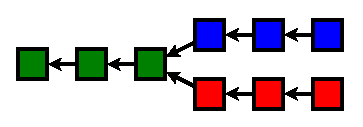
\includegraphics{figures/unl-clique-disjoint-blockchain.eps}
    \caption{Forked blockchain}
    \label{fig:unl-clique-disjoint-blockchain}
\end{figure}

\begin{figure}
    \centering
    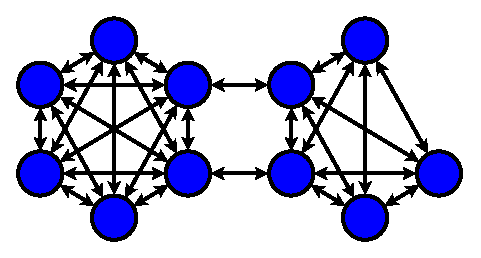
\includegraphics{figures/unl-clique-consensus.eps}
    \caption{UNL cliques in consensus}
    \label{fig:unl-clique-consensus}
\end{figure}

\begin{figure}
    \centering
    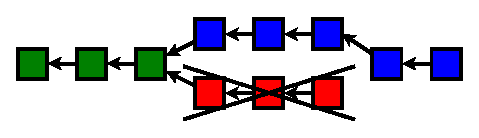
\includegraphics{figures/unl-clique-reorganized-blockchain.eps}
    \caption{Post-fork reorganization}
    \label{fig:unl-clique-post-fork}
\end{figure}


\subsection{Choosing the Unique Node List}

How should Ripple node administrators pick their Unique Node List? Ripple Labs
provides little, if any, concrete advice beyond the ``starter UNL'' they
provide. Let's look at this problem from another angle: Why shouldn't a node
operator just use the default UNL?

Let's assume the node operator does not know what UNL other nodes in the
economic majority have chosen to use. They do however know the default UNL
provided by Ripple Labs, and they have a reasonable belief that other node
operators also know that UNL and may also be using it. The node operator's goal
is to limit losses; the best case is their node stays in consensus with other
nodes. Second best is they suffer a denial of service attack causing their node
to stop processing some or all transactions. Worst case is their node accepts
transactions that other nodes do not, making possible double-spend attacks.
Table \ref{tbl:unl-outcomes} shows the outcomes of various possible
decisions by them and other node operators, ranging from $100\%$ default UNL,
$50\%$ default UNL, and $10\%$ default UNL.

In every circumstance node operators can reduce the risk of losses due to
consensus failures by removing non-default UNL entries, with the least risky
option being to simply stick with the default UNL of $100\%$ Ripple Labs
controlled nodes. This is particularly acute given the low profit margins of
many financial transactions: while a denial-of-service halts incoming revenue,
a double-spend attack can quickly drain working capital, quite possibly without
any hope of ever recovering the stolen funds.

A closely related issue is what incentive does a node operator have to publicly
perform validation services? Ripple currently has no compensation mechanism for
public validators, yet validation at minimum raises potential legal issues such
as lawsuits for negligence. Again, the least-risk option is to not publicly
validate the Ripple ledger.

\begin{table}
    \centering

    \begin{tabular}{cc|c|c|c}
        \multicolumn{2}{c}{} & \multicolumn{3}{c}{Majority} \\
        \multicolumn{2}{c}{} & $100\%$ & $50\%$ & $10\%$ \\ \cline{3-5}
        \multirow{3}{*}{Local} & $100\%$ & Consensus & DoS & DoS \\ \cline{2-5}
        ~ & $50\%$ & DoS & DoS & Doublespend \\ \cline{2-5}
        ~ & $10\%$ & Doublespend & Doublespend & Doublespend \\
    \end{tabular}

    \caption{Worst-case outcomes of default UNL \% choices}
    \label{tbl:unl-outcomes}
\end{table}


\section{Attack scenarios}

To evaluate potential attacks on the Ripple network we look at three factors:

\begin{itemize}

    \item \textbf{Type:} What is the effect of the attack? Denial of Service
          and/or theft? Or is the attack mostly useful in preparation for another
          type of attack?

    \item \textbf{Cost:} What is a probable minimum cost to carry out the attack, for
          the people able to do the attack? For instance, a technical attack
          that can be launched by ``bored teenagers'' will have an essentially
          zero cost while a long-term rewrite of a proof-of-work blockchain has
          a reasonably well-defined cost.

    \item \textbf{Scope:} Who is affected by the attack? Is this a targetted attack,
          mainly affecting a one or two targets? An attack with broad impact? Or
          an attack with global impact on all Ripple users?

    \item \textbf{Duration:} How long will it take before the attack is
          neutralized?  This may be a matter of hours to write and distribute a
          simple software patch\footnote{The author personally stopped the
          CVE-2013-4627 attack on the Bitcoin network in a few hours of rushed
          work in the middle of the night.}, to indefinitely long for some
          attacks where recovery is impossible.

    \item \textbf{Probability:} How likely is it for the Ripple network to be
          attacked this way?

\end{itemize}

We do \emph{not} try to determine the monetary impact of the attack, because we
are unable to predict how the Ripple network will be used. For instance, while
a double-spend attack may have the same basic impact on a $\$100/\text{day}$
small business as it would on a $\$1,000,000,000/\text{day}$ multinational, the
latter could lose orders of magnitude more money for what it at a technical
level basically the same attack. A closely issue with attempting to predict
monetary losses is that at some point losses can be sufficiently high that they
create situations where social consensus can decide that the losses simply must
be reversed. For instance, Vericoin community chose to do a hard-fork of their
alt-currency to undo the impact of a major theft.\cite{coindesk-vericoin}


big picture with attacks is there is not a minimum cost to them unlike PoW

evaluate attacks for denial-of-service and theft potential; evaluate minimum
cost to carry out attack; possible minimum manpower to carry out attack


Type of attack: DoS and/or theft

Minimum cost: $0, $1k, $10k, $100k

Scope: targetted, broad, global
Duration: hours, days, weeks, indefinite - How long will it take to fix the bug?

we don't attempt to put a dollar figure on harm done, as depends enormously on
how people use ripple


\subsection{Consensus Split}

The attacker exploits a difference in behavior between different
implementations/versions of the Ripple protocol. The result of the attack can
be a simple denial of service due to the Ripple network being unable to process
transactions, or with more sophistication, the attacker can fork the Ripple
ledger/blockchain and use the fork to doublespend. The attack is stopped by
identifying it, and then distributing software patches. Provided the Ripple
network is well monitored consensus split attacks can be stopped fairly
quickly; the March 2013 Bitcoin chain fork\cite{bip50} was resolved in a matter
of hours by contacting mining pools. A similar response could happen on Ripple
by contacting validating nodes commonly used in UNLs.\footnote{Another reason
to use the UNL provided Ripple Labs.}

Note that a consensus split may also happen by accident; prior consensus splits
in cryptocurrency systems have almost always been accidental. Equally, that
consensus splits can happen by accident clearly shows that the minimum cost to
perform this attack is zero. However, due to the limited number of consensus
bugs available to exploit in a given (set of) versions of the Ripple protocol
in use and the fast response time possible to consensus splits the potential of
this class of attack for long-term attacks on the network is limited.

Risk factors:

\begin{itemize}

    \item The main implementation of the Ripple protocol, \emph{rippled}, does
        not cleanly separate the consensus-critical part of the codebase from
        the non-consensus-critical part.\footnote{The consensus-critical
            portions of Bitcoin Core codebase are currently being separated
            into a stand-alone \emph{libconsensus} library.}

    \item The Ripple protocol itself is extremely complex, with many different
          types of transactions, and all functionality being implemented directly
          in the protocol itself.

    \item Improvements to Ripple frequently require changing the
          consensus-critical codebase rather than user software. For instance
          while on Bitcoin the implementation of multisig was possible without
          modification to the protocol\cite{bip19} in Ripple the lack of
          extension capabilities such as scripting require a consensus-critical
          change.\cite{ripple-wiki-multisign}\footnote{P2SH was \emph{not}
          required for multisig to be implemented.}

\end{itemize}

DoS: Cost \$0, Scope: global, Duration: hours, Prob: high
Theft: Cost \$1k, Scope: varies, Duration: hours, Prob: high

not as synergistic with other attacks; obvious flaw that will be fixed;
time-limited attack


\subsection{Transaction Flood}

DoS: Cost depends, Scope: broad, Duration: depends

The attacker creates large numbers of transactions - either covertely or
overtly - until the Ripple network fails due to overload, or more likely,
Ripple users are priced out of their ability to use the Ripple network.
Transactions pay a minimum fee per transaction by destroying XRP; the fee per
transaction is set by a vote between all validators on the UNL list. In the
short to medium term such an attack would quickly drive up that fee. A
succesful attack requires deep pockets as the attacker must outspend other
Ripple users.


Risk factors:

\begin{itemize}

    \item Ripple Labs plans\cite{cointelegraph-ripple-aml} to require verified
        user identification to use the Ripple network in the near future.  When
        implemented this will make it easy to determine who is doing a covert
        transaction flood attack and restrict their access to the network.

    \item The global consensus ledger has inherently poor $O(n^2)$ scaling;
        even in the absense of a malicious attack the poor scalability of the
        ledger is a threat to the viability of Ripple.

    \item A clever attacker wishing to overtly attack the Ripple network can
        masquerade their traffic as legit economic activity; from the point of
        view of Ripple Labs - a major XRP owner - such an attack may not even
        be considered an attack!\footnote{Similar to the debates in the Bitcoin
        ecosystem about whether or not fee-paying uses of the Bitcoin
        blockchain for non-Bitcoin-denominated transactions constitute
        ``attacks''.}

    \item Attacking the poor scalability of Ripple is highly synergistic with
        attacks depending on the high centralization of the Ripple network as
        even ``unsuccesful'' scalability attacks drive further centralization.
        For instance, if the response to a scalability attack is for Ripple
        Labs to beef up the validation nodes they control, and users stop
        running full nodes themselves, the network is more vulnerable to any
        attacks on those centrally managed validation nodes.

\end{itemize}




\subsection{UNL: Jurisdictional}

DoS/Theft: Cost \$100k, Scope: varies, Duration: indefinite

centralization attack - legal attack against centralized UNL. note
jurisdictional issues with delegating consensus to UNL

biggest issue is how can ripple compete against systems without the global
consensus req? if I'm a bank in russia, why use ripple when it opens me to UNL
issues?


\subsection{Software backdoor}

DoS/Theft: Cost \$0, Scope: varies, Duration: varies

mention unsigned code here


\subsection{UNL: key theft}

prep: Cost \$0, Scope: global, Duration: N/A

Gain control of UNL signing keys through theft/compromise. 


\subsection{Validator Fear, Uncertainty, and Doubt}

make people afraid to run validating nodes

illegal data


\subsection{History simulation}

Theft: Cost \$0, Scope: targetted, Duration: weeks

from proof-of-stake terminology; simulated history is costless as no work
expended.

use backdoored software as example of how this can happen; also can happen with
jurisdictional attacks

if rippled sees two versions of history, what happens?

rewrite history attack - note lack of cost to rewrite because no PoW; single
implementation so likely we can hack all nodes at once

proof-of-work has a hard bound on rewrite attacks, because can't break laws of
physics

can talk about how cost to do a simulation attack is PoW targets; talk about slasher rule


\section{Synergistic Attacks}

do a directed graph of likely synergistic attack sequences


\bibliographystyle{plain}
\bibliography{paper}

\end{document}
